\begin{figure}[ht]
\centering
    
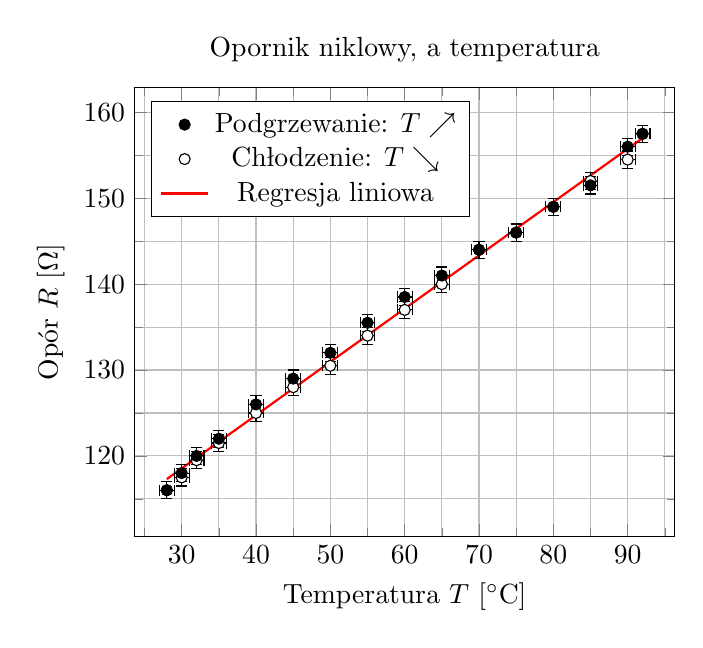
\begin{tikzpicture}
\begin{axis}[
    title={Opornik niklowy, a temperatura},
    xlabel={Temperatura $T$ [$^{\circ}$C]},
    ylabel={Opór $R$ [$\Omega$]},
    legend pos=north west,
    grid=both,
    minor tick num=1,
    % Tells pgfplots to skip over 'nan' entries safely
    unbounded coords=jump, 
    % Adjusts axis limits slightly so error bars aren't cut off
    enlarge x limits=0.05, 
    enlarge y limits=0.1,
]

\def\slope{0.62028}
\def\intercept{99.9313}
        
\addplot [red, thick, domain=28:92, forget plot] {\slope*x + \intercept};

% Cooling Data (↘ R_c) - Empty Symbols
\addplot [
    only marks,
    mark=*,
    color=black,
    forget plot,
    mark options={fill=white},
    error bars/.cd,
        x dir=both, x fixed=1,
        y dir=both, y fixed=1,
] table [x=T, y=R_down] {
    T     R_up  R_down
    28	116	116
    30	118	117.5
    32	120	119.5
    35	122	121.5
    40	126	125
    45	129	128
    50	132	130.5
    55	135.5	134
    60	138.5	137
    65	141	140
    70	144	144
    75	146	146
    80	149	149
    85	151.5	152
    90	156	154.5
    92	157.5	157.5
};

% Heating Data (↗ R_c) - Filled Symbols
\addplot [
    only marks,
    mark=*,
    color=black,
    forget plot,
    error bars/.cd,
        x dir=both, x fixed=1,
        y dir=both, y fixed=1,
] table [x=T, y=R_up] {
    T     R_up  R_down
    28	116	116
    30	118	117.5
    32	120	119.5
    35	122	121.5
    40	126	125
    45	129	128
    50	132	130.5
    55	135.5	134
    60	138.5	137
    65	141	140
    70	144	144
    75	146	146
    80	149	149
    85	151.5	152
    90	156	154.5
    92	157.5	157.5
};

\addlegendimage{only marks, mark=*, black, error bars/.cd, y dir=both, y explicit}
\addlegendentry{Podgrzewanie: $T \nearrow$}

\addlegendimage{only marks, mark=*, black, mark options={fill=white}, error bars/.cd, y dir=both, y explicit}
\addlegendentry{Chłodzenie: $T \searrow$}

\addlegendimage{no markers, red, thick}
\addlegendentry{Regresja liniowa}

\end{axis}
\end{tikzpicture}

\caption{
    Zmierzone opory opornika niklowego dla różnych temperatur wraz z niepewnościami pomiarowymi oraz prostą $R=aT+b$ doprasowaną przy pomocy regresji liniowej.
}
\label{img:opornik-nikolwy-wykres}
\end{figure}
